\textbf{A3 typos} \\
2c) \\
3b) $I(n-1)\mathrel{\overset{\geq}{\cancel{\leq}}}I(n-\tfrac12)\mathrel{\overset{\geq}{\cancel{\leq}}}$ \\
$\overset{\pi/2}{\cancel{\pi}}=\lim(\frac21\frac23\dotsm)$ \\
4a) $\frac{f'(k)-f'(k+1)}{4}$ \\
$\sum\log k=n\log n-n+\frac12\log n+c_n$ \\
$\overset{e^{c_n}}{\cancel{c_n}}\to\sqrt{2\pi}$

\textbf{Euler's Proof of Pentagonal Number Theorem} \\
\textbf{ref} Math Magazine \\
Vol 56 \#5, Nov 1983 \\
(by G.~Andrews) \\
G.~Polya Math \& Plausible Reasoning \\
Vol I

\thm
\[ \prod_{n=1}^\infty(1-x^n) = 1 + \sum_{n=1}^\infty (-1)^n(x^{n(3n-1)/2}+x^{n(3n+1)/2}) \]
\textbf{Sketch Proof:} Let
\begin{align*}
f(x,y) &= 1 - \sum_{n=1}^\infty (1-xy)(1-x^2y)\dotsm(1-x^{n-1}y)x^ny^{n+1} \\
&= \lim_{n\to\infty} f_l(x,y) \\
f_l(x,y) &= 1 - \sum_{n=1}^l (1-xy)(1-x^2y)\dotsm(1-x^{n-1}y)x^ny^{n+1}
\end{align*}
verify inductively that
\begin{align*}
f_l(x,1) &= (1-x)(1-x^2)\dotsm(1-x^l) \\
\text{so } f(x,1) &= \prod_{n=1}^\infty (1-x^n) .
\end{align*}
Verify that $f(x,y)$ satisfies the recursion formula (or functional equation)
\[ f(x,y) = 1 - xy^2 - x^2 y^3 f(x,xy) \]
Use this (repeatedly) to show that
\begin{align*}
f(x,y) &= 1 + \sum_{n=1}^{l-1}(-1)^n(x^{n(3n-1)/2}y^{3n-1}+x^{n(3n+1)/2}y^{3n}) \\
&\quad + (-1)^l(x^{l(3l-1)/2}y^{3l-1}+x^{l(3l+1)/2}y^{3l})f(x,xy^l)
\end{align*}
Let $l\to\infty$ then take $y=1$.
\[ \sum_{p\leq x}\frac{\log p}{p} \quad \sum_{p\leq x}\frac1p \quad \sum_{n\leq x}\frac{\Lambda(n)}{n} \]
\lem (Shapiro) Let $a\colon\Z^+\to[0,\infty)$. \\
If $\sum_{n\leq x}a(n)\floor{\frac xn}=x\log x+O(x)$ then $\sum_{n\leq x}a(n)\frac xn=x\log x+O(x)$ so $\sum_{n\leq x}\frac{a(n)}{n}=\log x+O(1)$. \\
\pf Suppose $\sum_{n\leq x}a(n)\floor{\frac xn}=x\log x+O(x)$
\begin{align*}
\text{Then } \sum_{n\leq x} a(n)\frac{x}{n} &= \sum_{n\leq x} a(n)\paren*{\floor*{\frac xn}+\chev*{\frac xn}} \\
&= \sum_{n\leq x} a(n)\floor*{\frac xn} + \sum_{n\leq x}a(n)\chev*{\frac xn} \\
&= x\log x + O(x) + \sum_{n\leq x}a(n)\chev*{\frac xn}
\end{align*}
and $\abs*{\sum_{n\leq x}a(n)\chev*{\frac xn}}\leq\sum_{n\leq x}a(n)$. \\
So if suffices to show that $\sum_{n\leq x}a(n)=O(x)$.

Let $S(x)=\sum_{n\leq x}a(n)$ and $T(x)=\sum_{n\leq x}a(n)\floor*{\frac xn}$.  Then
\begin{align*}
T(x) - 2T(\tfrac x2) &= \sum_{n\leq x}a(n)\floor*{\frac xn} - 2\sum_{n\leq\frac x2}a(n)\floor*{\frac x{2n}} \\
&= \sum_{n\leq\frac x2}a(n)\paren[\Big]{\underbrace{\floor*{\frac xn}-2\floor*{\frac x{2n}}}_{\in\brace{0,1}}} + \sum_{\frac x2<n\leq x}a(n)\floor*{\frac xn} \\ \intertext{
\begin{center}
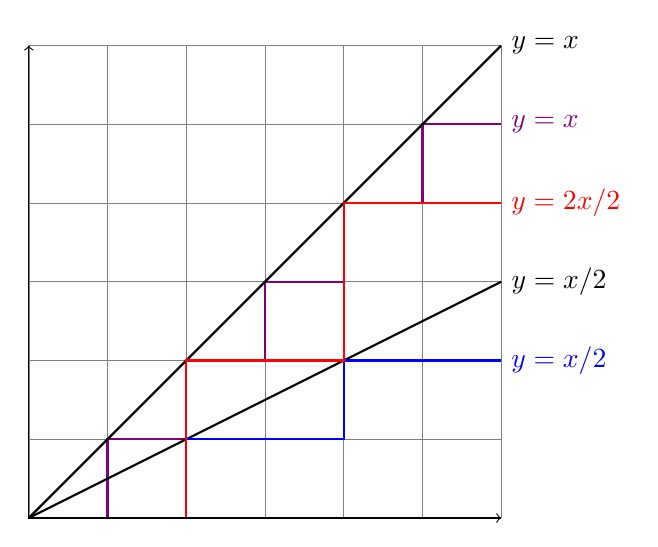
\begin{tikzpicture}
\draw[gray,very thin] (0,0) grid (6,6);
\draw[violet, thick, samples at={0,...,5,5.999},const plot] plot (\x, {floor(\x)}) node[right] {$y=\floor{x}$};
\draw[thick, domain=0:6] plot(\x, \x) node[right] {$y=x$};
\draw[thick, domain=0:6] plot(\x, \x/2) node[right] {$y=x/2$};
\draw[blue, thick,samples at={0,...,5,5.999},const plot] plot(\x, {floor((\x/2))}) node[right] {$y=\floor{x/2}$};
\draw[red, thick, samples at={0,...,5,5.999},const plot] plot(\x, {2*floor((\x/2))}) node[right] {$y=2\floor{x/2}$};
\draw[<->] (0,6) -- (0,0) -- (6,0);
\end{tikzpicture}
\end{center}
}
&\geq \sum_{\frac x2<n\leq x}a(n)\floor*{\frac xn} \\
&= \sum_{\frac x2<n\leq x}a(n) \\ \intertext{
since for $\frac x2<n\leq x$ we have
\[ \frac x2<n\implies \frac xn<2,\qquad n\leq x\implies \frac xn\geq1 \text{ so }\floor*{\frac xn} = 1 \]}
&= \sum_{n\leq x}a(n) - \sum_{n\leq\frac x2}a(n) \\
&= S(x) - S(\tfrac x2) \\
\therefore S(x) - S(\tfrac x2) &= T(x) - 2(\tfrac x2) \\
&= (x\log x+O(x)) - 2(\tfrac x2\log\tfrac x2 + O(\tfrac x2)) \\
&= (x\log x+O(x)) - (x\log x - x\log 2 + O(x)) \\
&= O(x)
\end{align*}
Choose $c>0$ so that $S(x)-S(\frac x2)\leq cx$ for large $x$, say $x\geq a$.  We have $S(x)=\sum_{n\leq x}a(n)$ for $x\geq1$ and we set $S(x)=0$ for $x<1$.
Modify $c$ so that $S(x)-S(\frac x2)\leq cx$ for all $x>0$ (since $S(x)$ is bounded for $1\leq x\leq n$).  Then we have
\begin{align*}
S(x) - S(\tfrac x2) &\leq cx \\
S(\tfrac x2) - S(\tfrac x4) &\leq \tfrac{cx}{2} \\
S(\tfrac x4) - S(\tfrac x8) &\leq \tfrac{cx}{4} \\
&\eqvdots
\end{align*}
eventually $S(\frac x{2^n})=0$.  Add those to get
\begin{align*}
S(x) &\leq cx(1+\tfrac12+\tfrac14+\dotsb) \\
&\leq 2cx \\
\therefore S(x) &= O(x)
\end{align*}
\eg Find an asymptotic formula for $\sum_{n\leq x}\frac{\Lambda(n)}{n}$
\[ \paren[\Big]{\text{where $\Lambda(n)=\begin{cases}
\log p & \text{when $n=p^k$ is a prime power} \\
0 & \text{otherwise}
\end{cases}$}} \]
\soln [incorrect?]
\begin{align*}
\sum_{n\leq x}\frac{\Lambda(n)}{n} &= \sum_{p^k\leq x}\frac{\log p}{p^k} \\
&= \sum_{p\leq x}\sum_{\substack{k\geq1\\p^k\leq x}}\frac{\log p}{p^k} \\
&= \sum_{p\leq x}\paren[\bigg]{\log p\sum_{\substack{k\geq1\\p^k\leq x}}\frac1{p^k}}
\end{align*}
\soln Consider $\sum_{n\leq x}\Lambda(n)\floor{\frac xn}$
\begin{align*}
\sum_{n\leq x}\Lambda(n)\floor*{\frac xn} &= \sum_{p^k}\log p\floor*{\frac x{p^k}} \\
&= \sum_{p\leq x}\log p\sum_{\substack{k\geq1\\p^k\leq x}}\floor*{\frac x{p^k}} \\
&= \sum_{p\leq m}\log p\sum_{k\text{ st }p^k\leq m}\floor*{\frac m{p^k}} \text{ where $m=\floor{x}$} \\
&= \sum_{p\div m!}(\log p) e_p(m!)\footnote{since $\floor*{\frac x{p^k}}=\floor*{\frac{\floor{x}}{p^k}}$} \\
\exp\paren[\Big]{\sum_{n\leq x}\Lambda(n)\floor*{\frac xn}} &= \prod_{p\div m!}\exp(e_p(m!)\log p) \\
&= \prod_{p\div m!}p^{e_p(m!)} = m! \\
\sum_{n\leq x}\Lambda(n)\floor*{\frac xn} &= \log(m!) = \log(\floor{x}!) \\
&= x\log x - x + \tfrac12\log x + O(1)
\end{align*}
By Shapiro's Lemma
\begin{gather*}
\sum_{n\leq x}\Lambda(n)\frac xn = x\log x+O(x) \\
\therefore \sum_{n\leq x}\frac{\Lambda(n)}{n} = \log x + O(1)
\end{gather*}
\ex Use this to get an asymptotic formula for
\[ \sum_{p\leq x}\frac{\log p}{p} . \]
\text{Challenging exercise:} Get an asymptotic formula for
\[ \sum_{p\leq x}\frac{1}{p} . \]
